\documentclass[UTF8]{ctexart}
\usepackage{lmodern}
\usepackage{amsmath}
\usepackage{graphicx}
\usepackage{float}%提供float浮动环境
\usepackage{booktabs}%提供命令\toprule、\midrule、\bottomrule
\usepackage{geometry}

\geometry{a4paper,left=2cm,right=2cm,top=2cm,bottom=2cm}

\title{{电子技术基础实验} \\ \textbf{实验一\ 常用测量仪器的使用}}
\author{\\\textbf{祝尔乐}
        \\\textbf{未央-电01}
        }
\date{\textbf{\today}}


\begin{document}
\maketitle


\section*{一.实验目的}

1. 熟悉示波器的使用,掌握用示波器测量交流信号的幅度、频率等参数,以
及测量脉冲波形的上升沿、下降沿等参数的方法。
2. 熟悉信号发生器的使用。

\section*{二.实验内容}

\subsection*{2.1 测量示波器的校准信号PROBE COMP}

测量结果如下表:
\begin{table}[H]
    \centering
    \caption{\label{表1}\textbf{测量示波器标准信号}}
    \begin{tabular}{ccc}
    \toprule
        & 峰-峰值/$V$ &  频率/$kHz$ \\
    \midrule
        自动测量 & 5.44 &  1.006 \\
        光标测量 & 5.42 &  1.005 \\
    \bottomrule
  \end{tabular}
\end{table}

% 自动测量 峰值:5.44V 平均值 2.54V 周期 995us 频率1.006kHz

\subsection*{2.2 用示波器测量正弦信号参数}
测量结果如下表:

\begin{table}[H]
    \centering
    \caption{\label{表2}\textbf{测量正弦信号参数}}
    \begin{tabular}{cccccc}
    \toprule
        上峰值/$V$ & 下峰值/$V$ & 峰-峰值/$V$ & 有效值/$V$ & 周期/$\mu s$ & 频率/$kHz$ \\
    \midrule
        0.520 & -0.528 & 1.10 & 0.35 & 100.0 & 10.00 \\
    \bottomrule
    \end{tabular}
\end{table}


\subsection*{2.3 测量不同频率下两正弦交流电压$v_i$和$v_o$}
电路图如下:
\begin{figure}[htbp]
    \centering
    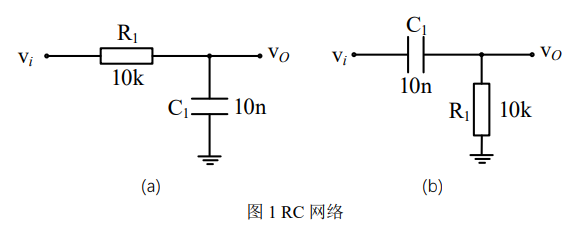
\includegraphics[width=0.60\textwidth]{3-电路图.png}
\end{figure}

分别在$10Hz-100Hz-1kHz-10kHz$的频率的$v_i$下测量$v_i$(设定$2VPP$)与$v_o$的有效值和相位差,
结果如下表:
(相位差测量方式: $\Delta \varphi = 2 \pi f \Delta t$ )

\begin{table}[H]
    \centering
    \caption{\label{表3}\textbf{正弦交流电下的电路参数测量}}
    \begin{tabular}{cccc|ccc}
    \toprule
                & (a)     &         &                           & (b)     &         &                           \\
        $f/kHz$ & $U_i/V$ & $U_o/V$ &  $\Delta \varphi / rad$ & $U_i/V$ & $U_o/V$ &  $\Delta \varphi / rad$ \\
    \midrule
        0.01 & 0.714 & 0.709 & 0.01 & 0.712 & 0.004& -1.81\\
        0.1  & 0.713 & 0.66 & 0.21 & 0.712 & 0.046 & -1.63\\
        1    & 0.712 & 0.41 & 0.72 & 0.714 & 0.28 & -1.01\\
        10   & 0.712 & 0.10 & 1.78 & 0.714 & 0.710 & -0.13\\

    \bottomrule
    \end{tabular}
\end{table}

画出(a)和(b)电路参数随着频率的变化曲线:

\begin{figure}[htbp]
    \centering
    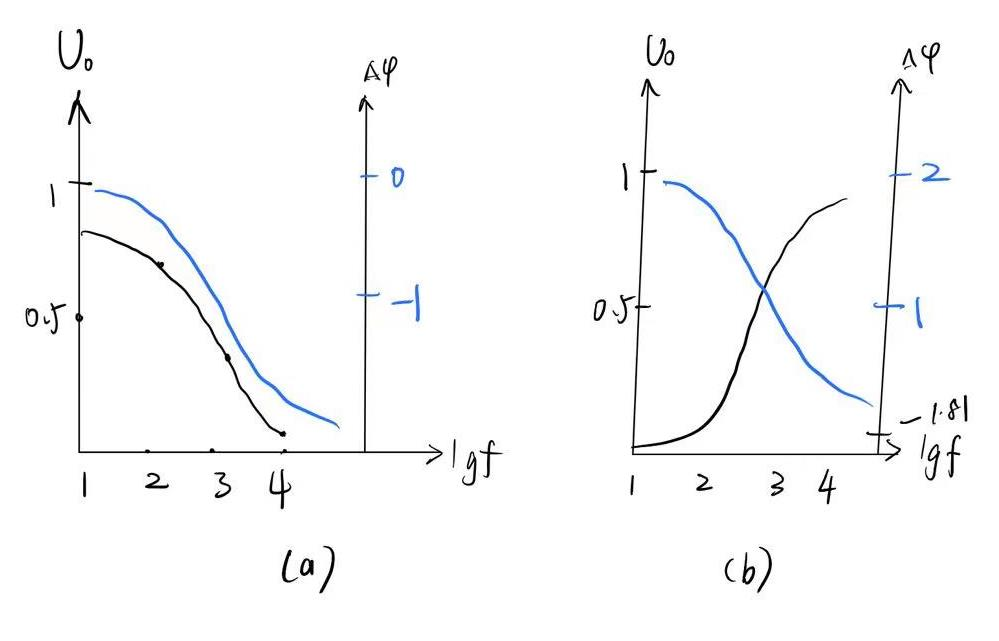
\includegraphics[width=0.40\textwidth]{2-3频率特性.jpg}
\end{figure}

从数据和图像可以看出,电路(a)的作用为低通滤波器,即可以通过频率较低的信号,频率较高的信号会被削弱;

电路(b)的作用为高通滤波器,即可以通过频率较高的信号,频率较低的信号会被削弱。

\subsection*{2.4 测量方波信号参数}

实验电路如图 1(a)所示,vi 是方波信号,幅度(即方波正半周电压)为 1VP,
频率为 500Hz, 测量 vi 与 vo 的波形及其上升时间 tr、下降时间 tf。

图像如下:
\begin{figure}[htbp]
    \centering
    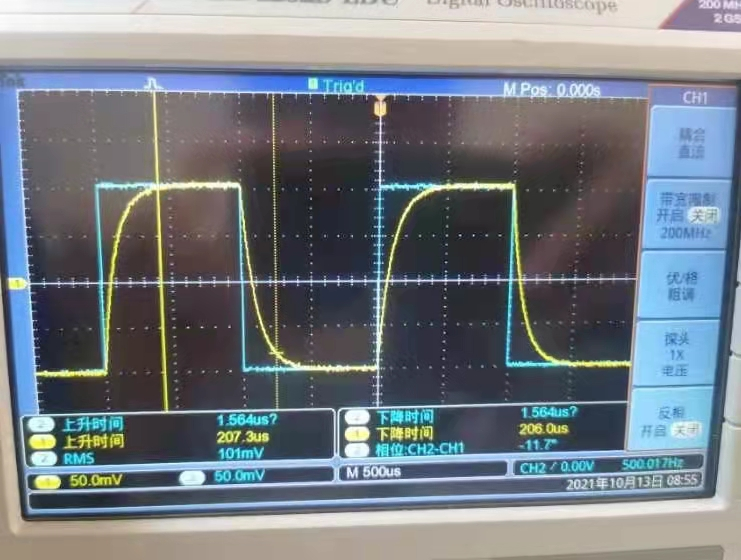
\includegraphics[width=0.40\textwidth]{方波-输入输出.jpg}
\end{figure}

测量结果如下:
\begin{table}[H]
    \centering
    \caption{\label{表4}\textbf{方波信号参数}}
    \begin{tabular}{ccc}
    \toprule
            &$t_r/\mu s$ & $t_f/ \mu s$  \\
    \midrule
            $v_i$ & 1.56 & 1.56 \\
            $v_o$ & 207 & 206 \\
    \bottomrule
    \end{tabular}
\end{table}

可以看出经过大电容的方波信号出现了"失真",即上升和下降的过程被放大了。

\subsection*{2.5 电路级联}
将(a)(b)的电路级联后测量电路参数。

级联后的结果如下:
\begin{table}[H]
    \centering
    \caption{\label{表5}\textbf{正弦交流电下的级联电路参数测量}}
    \begin{tabular}{cccc}
    \toprule
        $f/kHz$ & $U_i/V$ & $U_o/V$ &  $\Delta \varphi / rad$ \\
    \midrule
        0.01 & 0.712 & 0.01& --\\
        0.1  & 0.712 & 6.4 & 1.48\\
        1    & 0.713 & 23.0 & 0.36 \\
        10   & 0.712 & 10.3 & -0.67 \\

    \bottomrule
    \end{tabular}
\end{table}

画出电路参数随频率变化的图像:

\begin{figure}[htbp]
    \centering
    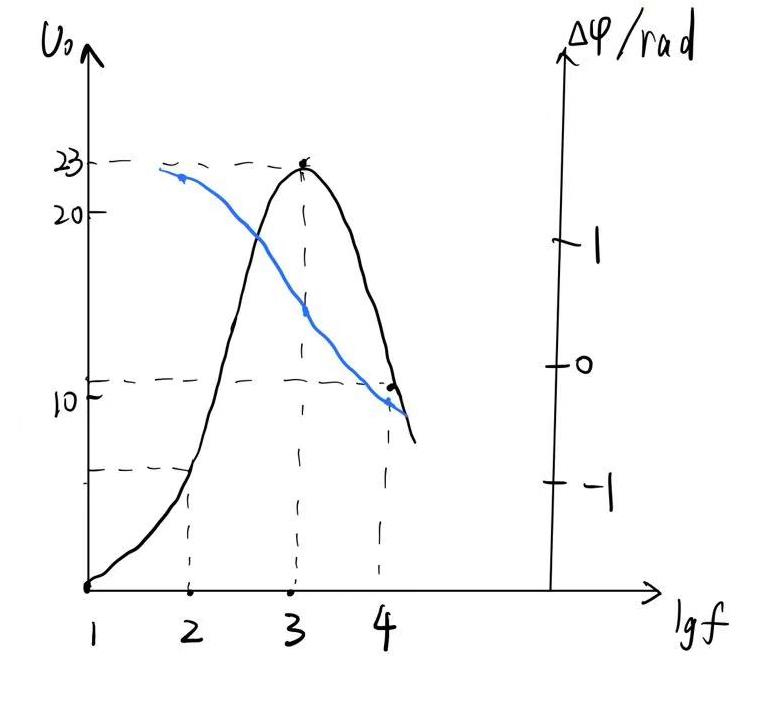
\includegraphics[width=0.40\textwidth]{2-5频率特性.jpg}
\end{figure}

从数据和图像可以看出,级联后的电路为带通滤波器。即对于高频(>10kHz),以及低频(<100Hz)的信号,
电路通过的信号幅值较小,而对于中间的频率段(100-10kHz)的信号,电路通过的信号幅值较大,
即电路具有带通特性

\subsection*{2.6 探究电路作用}

\begin{figure}[htbp]
    \centering
    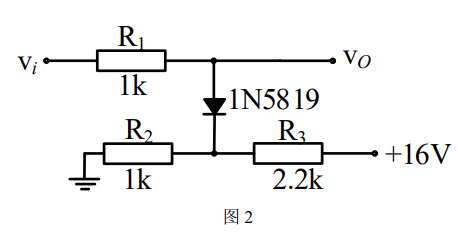
\includegraphics[width=0.40\textwidth]{6-电路图.png}
\end{figure}

搭建图2所示电路,vi 输入正弦波信号(1kHz),调节其幅值分别为10VPP,
15VPP,观察 vo波形变化;在R2上并联一个 10uF 电容,观察v0波形变化。

% \begin{figure}[htbp]
%     \centering
%     \includegraphics[width=0.80\textwidth]{6-10VPP-无电容.png}
% \end{figure}
% \begin{figure}[htbp]
%     \centering
%     \includegraphics[width=0.80\textwidth]{6-15VPP-无电容.png}
% \end{figure}
% \begin{figure}[htbp]
%     \centering
%     \includegraphics[width=0.80\textwidth]{6-10VPP-有电容.png}
% \end{figure}
% \begin{figure}[htbp]
%     \centering
%     \includegraphics[width=0.80\textwidth]{6-10VPP-有电容.png}
% \end{figure}

由图可以看出电路的作用将输入电压的瞬时值控制在$5V$以下,加入大电容的作用
是使得$R_2$的电压更加的稳定。


\subsubsection*{改进思路}
由于二极管在正向导通的时候仍然有一定的电压(不妨设为0.7$V$),于是实际控制
的电压最大值并不是我们想要的$5V$,而可能是$5.7V$,我们可以针对二极管对电阻
进行一定的调整。设二极管导通后的电压为$U_D$,则为了使得电压满足预期,$R_3$满足的方程:
\begin{align}
    U_{set} = \frac{R_2}{R_2 + R_3'}16 + U_T
\end{align}

令$R_2= 1k\Omega$,解得$R_3' = 2.72k\Omega$。

同样的,如果我们想得到一个限压5V(绝对值)的信号,那么二极管应该再并联一个方向与之相反的相同的二极管,
这样限压特性才是对称的,不会得到一个只是一边限压,另一边为正常正弦波的不对称波形。

\end{document}